
% Cal Poly Thesis
% 
% based on UC Thesis format
%
% modified by Mark Barry 2/07.
%




\documentclass[12pt]{ucthesis}

\newif\ifpdf
\ifx\pdfoutput\undefined
    \pdffalse % we are not running PDFLaTeX
\else
\pdfoutput=1 % we are running PDFLaTeX
\pdftrue \fi

\usepackage{url}
\ifpdf

    \usepackage[pdftex]{graphicx}
    % Update title and author below...
    \usepackage[pdftex,plainpages=false,breaklinks=true,colorlinks=true,urlcolor=blue,citecolor=blue,%
                                       linkcolor=blue,bookmarks=true,bookmarksopen=true,%
                                       bookmarksopenlevel=3,pdfstartview=FitV,
                                       pdfauthor={!!Author goes here!!},
                                       pdftitle={!!Title goes here!!},
                                       pdfkeywords={thesis, masters, cal poly}
                                       ]{hyperref}
    %Options with pdfstartview are FitV, FitB and FitH
    \pdfcompresslevel=1

\else
    \usepackage{graphicx}
\fi

\usepackage{amssymb}
\usepackage{amsmath}
\usepackage[letterpaper]{geometry}
\usepackage[overload]{textcase}
\usepackage{subfig}
\usepackage{float}


\bibliographystyle{abbrv}

\setlength{\parindent}{0.25in} \setlength{\parskip}{6pt}

\geometry{verbose,nohead,tmargin=1.25in,bmargin=1in,lmargin=1.5in,rmargin=1.3in}

\setcounter{tocdepth}{2}
\graphicspath{{fig/}}


% Different font in captions (single-spaced, bold) ------------
\newcommand{\captionfonts}{\small\bf\ssp}

\makeatletter  % Allow the use of @ in command names
\long\def\@makecaption#1#2{%
  \vskip\abovecaptionskip
  \sbox\@tempboxa{{\captionfonts #1: #2}}%
  \ifdim \wd\@tempboxa >\hsize
    {\captionfonts #1: #2\par}
  \else
    \hbox to\hsize{\hfil\box\@tempboxa\hfil}%
  \fi
  \vskip\belowcaptionskip}
\makeatother   % Cancel the effect of \makeatletter
% ---------------------------------------




\begin{document}

% Declarations for Front Matter

% Update fields below!
\title{Spatial Reasoning in Architectural Design}
\author{Gregory Flanagan}
\degreemonth{September} \degreeyear{2010} \degree{Master of Science}
\defensemonth{September} \defenseyear{2010}
\numberofmembers{3} \chair{Franz Kurfess, Ph.D.} \othermemberA{Mehul Bhatt, Ph.D.} \othermemberB{John Seng, Ph.D.} \field{Computer Science} \campus{San Luis Obispo}
\copyrightyears{seven}



\maketitle

\begin{frontmatter}

% Custom made for Cal Poly (by Mark Barry, modified by Andrew Tsui).
\copyrightpage

% Custom made for Cal Poly (by Andrew Tsui).
\committeemembershippage

\begin{abstract}
CAD systems lack the technology to capture and represent underlying building design
knowledge beyond purely geometrical information. The common thread of the work
 discussed here, are ways to capture, represent, and reason about building design
knowledge for use in creating intelligent building design systems.  



\end{abstract}

%\begin{acknowledgements}

%   Thank you...

%\end{acknowledgements}


\tableofcontents


\listoftables

\listoffigures

\end{frontmatter}

\pagestyle{plain}




\renewcommand{\baselinestretch}{1.66}


% ------------- Main chapters here --------------------





\chapter{Introduction}
\label{intro}


This is the introduction.



\chapter{Preliminaries}
\label{preliminaries}

\section{Qualitative Spatial Representation and Reasoning}
\subsection{Applications of Spatial Reasoning}
\subsubsection{Architectural Design}
\subsubsection{Geographic Information Systems}
\subsubsection{Robotics}
\section{Constraint Logic Programming}


\chapter{Previous Work}
\label{previous-work}
\section{Design Support Systems}
\subsection{SEEDS}
The SEEDS project, described in \cite{FlemmingIKM94}, proposed a architectural design platform for capturing and representing functional (i.e. spatial requirements) and structural (geometric) design knowledge. The aim of which is to support the architectural design process by providing design knowledge during the initial design phase of a building. Within the SEEDS project, design knowledge is partitioned into two categories: design units, and functional units. Design units represent spatial and physical elements of a building, while functional units represent requirement that constrain design units
based on shape, size, placement, etc.. Additionally, SEEDS pioneered the idea that architectural design knowledge, specifically design requirements, could be represented as constraints to automatically generate layouts.



\section{AI in Design}
\subsection{Intelligence Virtual Environments}
Caldern \cite{CalderónCLP06} built upon the ideas in \cite{FlemmingIKM94} for representing design knowledge, to develop an Intelligent Virtual Environment that solves spatial configuration problems based on spatial design knowledge. Additionally, the tool added non-geometric semantics (i.e. environmental, lighting) for functional units to demonstrate that their approach could be extended to non-geometric design knowledge.

Caldern argued that spatial knowledge By representing design knowledge as constraints, the tool was able to use constraint logic programming to solve spatial configuration problems. In general, constraint are classified as: topological, local, and global. Topological constraints describe the topological characteristics of the environment, such as a regions where a lighting is less then 300 lux. Local constraints describe the attributes of a
single object and how it interacts with topological characteristics. In general these characteristics are in the form of, a desk should be at least 4 meters from a ventilation duct, or an object should be within an area that has more then 300 lux of light. Global constraints express design requirements for a group of objects.  

Axling \cite{AxlingEURO96} and Codognet \cite{CodognetDMS99} proposed the use constraint  logic programming in Virtual Environments for intelligent object behavior. Their approaches focuses on the behavior of single objects without taking into consideration behavior of a set of object or how objects constrained by the specific environment. 

\subsection{V-SIMSPLACE}
\cite{LertlakkhanakulIBPSA06} describes a platform that 'embodies spatial context-aware information' so that users can visualize an architectural design before it is deployed. The aim of the tool is to simulate a users experience in a Smart Home environment, in order to study the interactions of the user within his/her environment. The crux of the system is that behavioral semantics of a Smart Home are integrated into the building design knowledge so that the interactions a user has within the Virtual Environment will closely mimic the real world.

Unlike \cite{CalderónCLP06}, V-PLACESIMS does not attempt to capture design requirements or reason about the consistency of an environment. Rather, it's focus is providing a platform for users to interact with a Smart Home environment to discover the behaviors and interactions that take place.

\subsection{Intelligence for Ambient Design}
Bhatt proposed a system in \cite{BhattDH09} that provides validation for the satisfiability of functional requirements, which are grounded to a qualitative spatial calculi, within the Ambient Environment domain. The system accomplishes this by modeling the functional requirements as constrains in an ontology and uses an ontology reasoner to discover if a model is realizable for a design, i.e. no models will be found if on or more functional constraints are not satisfied. 

\subsection{Decision Support for Virtual Environment}
\cite{Nomura92} used a Decision Support System to validate the design configuration. The system was used more as a diagnostic system, rather then providing feedback on how to reconfigure the environment. Note: I have not read \cite{Nomura92} because I haven't been able to track it down. Therefore my description here is based on the related works section of \cite{CalderónCLP06}.



\chapter{DSpace Reasoner}
The DSpace Reasoner is a prototype tool for validating conceptual design requirements against CAAD based architectural design plans. Conceptual design requirements here refer to requirements as they pertain to the functional and experiential aspects of the design from a semantic and qualitative perspective. For example, architects commonly describe aspects of a design in a qualitative fashion, such as a design being private, accessible, or continuous. These architectural aspects emerge from the spatial structures / arrangements of the building form and are experienced in the building. 

The goal of the DSpace reasoner is to build a computational framework to represent and reason about conceptual design requirements to validate conceptual design requirement to the real world, CAAD based architectural plans.     


\section{Design Problem}

to do this dspace need to:
 - representation of design
 	- spatial abstraction / multiple perspectives
 	- artefacts
 - design requirements - define / identify
 	- define architectural qualities
 		- perceptual
 		- intrinsic / geometric
 	- define architectural concepts
	- spatial interpretation / explicit characterization
 - qualitative spatial reasoning
 	- topological 
 	- orientation
 		- intrinsic vs extrinsic
 	- distance


\section{DSpace: Design and Implementation}


\chapter{Representation of Architectural Designs in DSpace}
\section{Multiple Perspectives and Spatial Abstraction}
\section{Artefacts}
\section{IFC / ArchiCAD import}

\chapter{Spatial Reasoning in Constraint Logic Programming Framework}
The spatial reasoning module in DSpace is built in a constraint logic programming framework. 

Constraint Handling Rules

Qualification

\section{Topology}
Topological reasoning works over points, lines, and regions (convex hulls). The main form of spatial topological reasoning is qualification. The following are the topological relationships that can be qualified: partially overlapping, ntpp, ntppi, disconnected and equals. 

Topological qualifications uses properties of line intersections and convex hulls to detect topological relationships. Constraint handling rules are used to simplify topological constraints until a simple constraint of line intersection checking and point / convex hull containment. The partially overlapping relationship is detected if and lines intersect between objects and 

\section{Orientation}

\subsection{Intrinsic Orientation}
OPRA
Relationships
  - i, j

Geometric Detection
  - partition of space in to half planes
  - linear inequalities

\subsection{Extrinsic Orientation}
SCC
Relationships
  - SCC rel
  
Geometric Detection
  - partition of space into half planes
  - linear inequalities

\section{Distance}
Uses Sindalog reasoner's distance constraints
Variation of distance constraints

\section{Sample Queries}
Examples with shapes
Examples with architectural elements in the DSpace reasoner


\chapter{Conceptual Design Requirements}
TBD: heuristic / explicit characterization / experience / common sense

TBD: spatial abstraction so attributes are not precise. Some fringe cases are pointed out, but all such cases are not identified and handled.

TBD - needs work: Thes attributes can be used to build together to build conceptual design requirements.

\section{Qualitative Spatial Attributes in Architecture}
This section presents a set of qualitative spatial attributes found in architecture and shows how they are spatially interpreted and represented in DSpace. These attributes are architectural qualities that are emerge from the spatial relationships and configurations between the spatial elements of the structural building (doors, walls, windows, etc.) and interior design (furniture, lights, decorations, etc.). Attributes can be perceptual, qualities that are described from a specific vantage point, or intrinsic, qualities that are inherent in the build's spatial structure. The goal of this section, is to develop a tool-kit of qualitative attributes that describe an architectural design in the spatial environments they emerge in. 

The set of qualitative spatial attributes developed in the section were taken from architectural design textbooks \cite{TBD}, museum research on visitor behaviour \cite{TBD}, and building codes \cite{TBD}. The objective here is not to develop an exhaustive list of qualitative spatial attributes for architecture or a validation of the interpretation of the attributes, rather it is to demonstrate a computational framework in which these qualities can be represented and used to reason about architectural design requirements.

\subsection{Facing}
The facing attribute defines an intrinsic orientational relationship between two objects as each relates to the other. The definition used here is based on a common sense interpretation of facing, in which an object \emph{A} is facing towards an object \emph{B}, if object \emph{B} is in front of object \emph{A} and object \emph{A} is directionally oriented at object \emph{B}. Under this definition, a pair of objects can be facing towards or away from each other. Given a pair of objects,\emph{A} and \emph{B}, there are four possible facing configurations between the pair: 

\begin{figure}[H]
 \centering
 \subfloat[A, B towards]{\label{fig:facing-towards}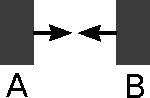
\includegraphics[width=25mm]{facing-towards}}
 \hspace{10 mm}
 \subfloat[A, B away]{\label{fig:facing-away}
\includegraphics[width=28mm]{facing-ABaway}}
  \hspace{10 mm}
 \subfloat[A towards, B away]{\label{fig:facing-A}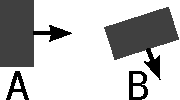
\includegraphics[width=28mm]{facing-Atowards-Baway}}
 \hspace{10 mm}
 \subfloat[A away, B towards]{\label{fig:facing-A}
\includegraphics[width=28mm]{facing-Aaway-Btowards}}
 \caption{facing}
\label{display-arrangement}
\end{figure}

The facing attribute is modelled in the DSpace reasoner using the Oriented Point Relation Algebra \cite{Moratz} (OPRA). The advantage of using OPRA is that it models the intrinsic orientational relationships between pairs of directed points. OPRA partitions space into half planes, which are defined by lines emanating outwards from the reference point, and defines the qualitative orientational relationships by the half plane in which a second point is located. Figure \ref{facing-opra-base-rel} shows the partitioning of space with labels for base relationships in OPRA$_{4}$. A second point is located in sector 6 of the partitioning scheme, so that the second point has an OPRA$_{4}$ 6 relationship with the point. Note that the arrow depicts the point's direction and the sectors are labelled starting in the point's direction and incrementing counter-clockwise. 

\begin{figure}[H]
\centering

\includegraphics[width=40mm]{facing-opra-base-rel}
\caption{OPRA$_{4}$ Space Partitioning}
\label{facing-opra-base-rel}
\end{figure}

Using OPRA$_{4}$, the facing attribute can be defined in terms of the half plane sectors. Point \emph{A} is facing towards point \emph{B}, if point \emph{B} is located in sectors 1, 2, or 16 of point \emph{A's} partitioned space. Similarly, if point \emph{A} is located in sectors 1, 2, or 16 of point \emph{B's} partitioned space then point \emph{B} is facing towards point \emph{A}. In this case points, both points are facing towards each other. Figure \ref{fig:facing-opra-towards} shows an example of two points facing towards each other; note that each point is located in sector 16 of the other's partitioned space. Conversely,  point \emph{A} is facing away from point \emph{B} if point \emph{B} is located in sectors 3 - 15 of point \emph{A's} partitioned space. Figure \ref{fig:facing-opra-away} shows an example of two points that are facing away from each other and are located in sectors 11 and 7. 

\begin{figure}[H]
 \centering
 \fbox{
 \subfloat[facing towards]{\label{fig:facing-opra-towards}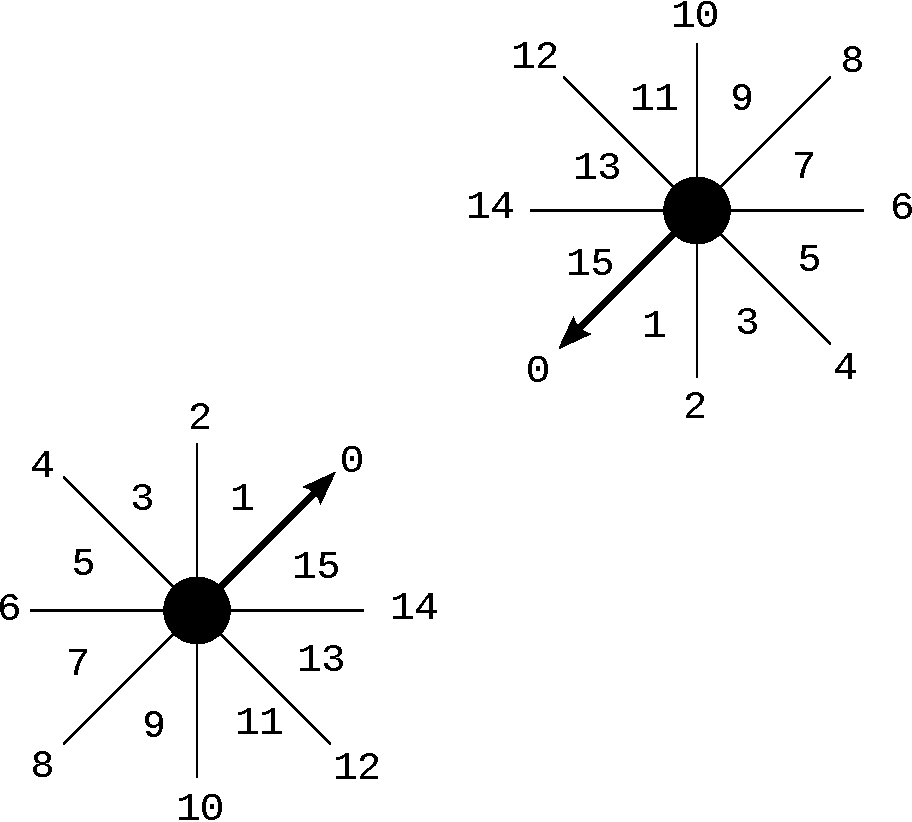
\includegraphics[width=60mm]{facing-opra}}
 }
  \hspace{10 mm}
  \fbox{
 \subfloat[facing away]{\label{fig:facing-opra-away}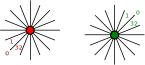
\includegraphics[width=60mm]{facing-away-opra}}
 }
 \caption{OPRA Partitioning }
\label{opra-facing}
\end{figure}

In DSpace, the facing attribute is represented as several predicates that take two arguments in the head of the clause. These arguments are the objects that will be check for the facing attribute. The body of the predicate defines logically, via conjunction and disjunction, the attribute based on the spatial definition given above.

\begin{verbatim}
   facing_towards(Obj1, Obj2) :- (opra(Obj1, Obj2, 1) ;
                                  opra(Obj1, Obj2, 2) ;
                                  opra(Obj1, Obj2, 16)).
                                 
   facing_away(Obj1, Obj2) :- (opra(Obj1, Obj2, 3) ;
                               opra(Obj1, Obj2, 4) ;
                               opra(Obj1, Obj2, 5) ;
                               opra(Obj1, Obj2, 6) ;
                               opra(Obj1, Obj2, 7) ;
                               opra(Obj1, Obj2, 8) ;
                               opra(Obj1, Obj2, 9) ;
                               opra(Obj1, Obj2, 10) ;
                               opra(Obj1, Obj2, 11) ;
                               opra(Obj1, Obj2, 12) ;
                               opra(Obj1, Obj2, 13) ;
                               opra(Obj1, Obj2, 14) ;
                               opra(Obj1, Obj2, 15)).
                                  
\end{verbatim}

In DSpace, the facing attribute can be used to check if two architectural structures and / or interior design objects are facing towards or away from the other. As an example, doorways and windows that face towards the other promote air flow through the room in which that they inhibit. A design requirement that promotes air circulation could include the use of windows and doorways that face towards each other. Figure XXX shows and example room where a window and door face each other. Additionally, the facing attribute can be used to build requirements between interior design element, such as desks, chairs, and beds as they related to windows, and doorways and other interior design elements. For example, an interior design requirement might be that a computer desk should not face towards a window, in order to reduce glare on the computer screen from direct sunlight. 

\begin{figure}[H]
 \centering
 \subfloat[facing towards]{\label{fig:door-window-towards}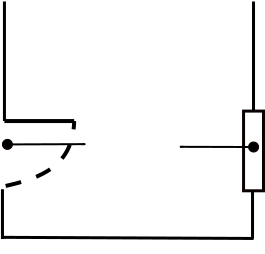
\includegraphics[width=55mm]{door-facing-window-con}}
  \hspace{10 mm}
 \subfloat[facing away]{\label{fig:door-window-away}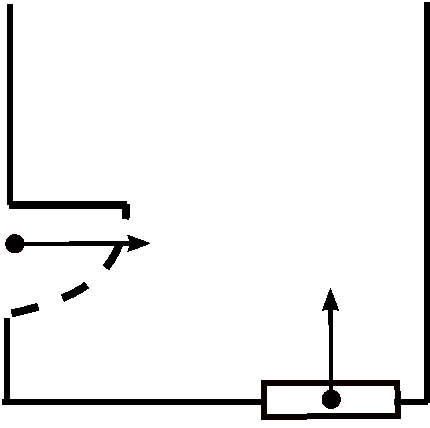
\includegraphics[width=53mm]{door-facing-window-incon}}

 \caption{Door, Window Facing}
\label{door-window-facing}
\end{figure}

Within the context of architecture, care needs to be taken to account for architectural structures that are long in one axis, such as walls, because the orientational spatial abstraction for OPRA is a directed point. This means that an object is facing a wall only if if is facing the wall's directed point abstraction. Under this definition, there are configurations where an object should be considered to be facing a wall but it is not. DSpace handles this special case by modifying the OPRA relationships that correspond to facing towards and away from. 

fig: wall example

\subsection{Proximity / Distance}
The proximity attribute defines a qualitative distance relationship between two objects. In DSpace there are two proximity relationships: near and far. The spatial interpretation of these relationships depends on the context and scale in which the objects inhibit. For the purposes here, and in the context and scale of architectural space, proximity is defined using heuristics based on the scale of building elements, i.e. rooms, apartments, buildings.

\begin{figure}[H]
\centering
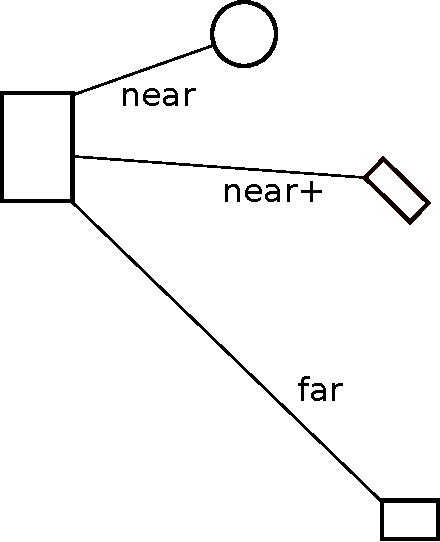
\includegraphics[width=45mm]{proximity}
\caption{proximity}
\label{proximity}
\end{figure}

Using these heuristics, two objects are near to each other if the minimum distance between them is less then or equal to 3 meters. Conversely, two objects are far away from each other if the minimum distance between them is greater then 3 meters. While the definition of proximity pivots around 3 meters, it can easily be change by using an extra parameter in a proximity predicate. 

In DSpace, proximity is represented as two predicates (near, far) each with two arguments in the head of the clause. The arguments that will be checked for proximity. The body of the clause defines the distance constraint that defines proximity.

\begin{verbatim}
   near(Obj1, Obj2) :- minimum_distance_compare(Obj1, Obj2, <=, 3).
   
   far(Obj1, Obj2) :- minimum_distance_compare(Obj1, Obj2, >, 3)

\end{verbatim}

The proximity attribute can be used to check if two architectural structures and/or interior design objects are near or far. For example, a computer desk should be located near a power outlet to make it easy to power up the computer and desk lamp. Another example is the bathroom should be far away from the kitchen, so to keep a separation between the two.

TBD: fig example


\subsection{Positioning}
The positioning attribute defines an orientational relationship between a pair of objects as each object relate to the other, within an extrinsic context, i.e. a defined space such as a room, apartment, building, or user defined space. There are four positioning relationships using this scheme: opposing-side of space, same-side of space, left-side of space, and right-side of space. The opposing-side and same-side relationships can be combined, via conjunction, with the left-side or right-side relationships to form the following compound relationships: opposing-left-side, opposing-right-side, same-left-side, same-right-side.

\begin{figure}[H]
\centering
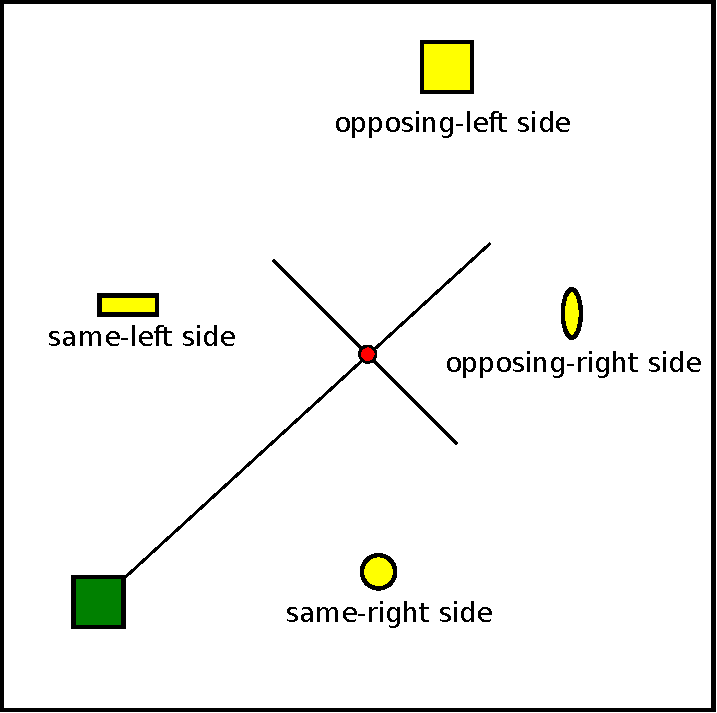
\includegraphics[width=60mm]{position}
\caption{Positioning}
\label{position}
\end{figure}

The positioning attribute is interpreted spatially in DSpace using the Single Cross (SCC) orientation calculus \cite{Freksa}. SCC defines the orientation of a point C (referent) with respect to a point B (relatum) from the viewpoint of a point A (origin). The positioning attribute uses the SCC scheme to relate two points (origin, referent) in the context of an external frame of reference (the relatum). In this case the relatum is a central point of the context space. In DSpace, the reference point is defined as the centroid of the space. The assumption here is that the context space will be generally rectangular in space (rooms, buildings, etc.).

TBD fig: SCC

Under this scheme, two points are define as being on opposing sides of a space if they have an SCC relationship of 0, 1, 7, as related by the centroid of the context space. Conversely, a pair of points are defined to be on the same side of the room if they have and SCC relationship of 2 - 6 as related by the centrod of the context space. On object is on the left side of the room from if it has an scc relationship of 0 -4, and right side if it has an scc relationship of 5 - 7. 

TBD fig:opposing / same / left /right side of space as defined in SCC

In DSpace, the positing attribute is represented in Prolog as several predicates with three arguments. The first two arguments are the objects that are being related and the third is the context space. The body of the clause defines the positing relationship logically based on the SCC interpretation given above.

\begin{verbatim}
   opposing_side(Obj1, Obj2, Context) :- centroid(Context, centroid),
                                         (scc(Obj1, centroid, Obj2, 0);
                                          scc(Obj1, centroid, Obj2, 1);
                                          scc(Obj1, centroid, Obj2, 7)).
                                          
   same_side(Obj1, Obj2, Context) :- centroid(Context, centroid),
                                     (scc(Obj1, centroid, Obj2, 2) ;
                                      scc(Obj1, centroid, Obj2, 3) ;
                                      scc(Obj1, centroid, Obj2, 4) ;
                                      scc(Obj1, centroid, Obj2, 5) ;
                                      scc(Obj1, centroid, Obj2) 6)).   

\end{verbatim}

The positioning attribute can be used to check if two architectural elements or interior design object are on the opposing or same side of a space to the other. For example, a requirement might state that a bedroom should be positioned to the bad of a house from the main entrance. The reason for this requirement is that rooms that are in the back of a house are more private than rooms in the front of the house. In this requirement, the origin is the entrance, the referent if the bedroom, and the relatum is the centroid of the house (context space).

TBD: fig:room back of house

\subsection{Visibility}
The visibility attribute defines a boolean relationship between a viewpoint and an object with respect to the object being visible from the viewpoint. An objects is visible if the view space in-between the viewpoint and the object is not obstructed. It should be noted that this definition of visibility does not take into account effects of distance on visibility, i.e. an object that is very far away is not visible. However, within the context of a architecture and buildings, the magnitude of distances is limited and in general is not a factor in visibility.

The spatial interpretation of visibility is based on the topological characteristics of the space in-between the viewpoint and object. This space is referred to as the view-space. An object is visible if the view-space is not obstructed by any surrounding structures or objects. An obstructing object is object that has a 
partially overlapping or containment topological relationship with the view-space. This definition does not decipher between a view that is partially or totally obstructed.

TBD fig:visibility

In DSpace visibility is represented as a predicate with two arguments in the head. The arguments are the viewpoint and an object. The body of the clause calculates the view-space in-between the viewpoint and object and checks the surrounding structures and objects for topological relationships.

\begin{verbatim}
   is_visible(ViewPoint, Obj) :- view_space(ViewPoint, Obj, ViewSpace),
                                 topology(ViewSpace, SurroundingStructs).
\end{verbatim}

The visibility attribute can be used to check if an architectural element is visible from a given viewpoint. For example, an architect might want to ensure that a certain staircase is visible from the main entrance because she doesn't want the staircase to go unnoticed. Figure XXX shows ....  


\subsection{Alignment / Symmetry}
The alignment attribute defines 

\subsection{Pathways / Turns}  right turn (hard) / left turn (hard) / straight 


\section{Architectural Concepts}
Architectural concepts such as privacy, continuity, and enclosure, which describe an experiential aspect of architecture as used by an architect to describe the functionality of a building \cite{Koile}. These terms are defined, in DSpace, in a hierarchical manner in which architectural concepts are defined by logically combining, via conjunction and disjunction, architectural qualities (i.e. previous section) and geometric primitives (orientation, topology, distance). 

This section defines four architectural concepts and demonstrates how they can are defined in DSpace. As in the previous section, the purpose here is not to investigate the correctness of the concepts or an attempt to look at a complete list of these concepts, rather it's to look at how these concepts cab be defined logically using architectural qualities and spatial / geometric primitives.

\subsection{Privacy}
The concept of privacy in architecture implies a notion of separation and obscurity (not being visible). In the case of a room, privacy can be defined as being separated from the main entrance of the building and having doorways which enhances the room's privacy. A doorway can be be defined as private with respect to its functionality of connecting two areas (rooms, hallways, etc.) together. With this consideration, a doorway can enhance or hinder the privacy of a room. A doorway enhances privacy if the doorways faces away from other local doorways and if it is not visible from the main living space. 

Within DSpace, the concepts of privacy has been formally defined for rooms and doorways. A door is private if it has the following attributes: (1) it is not visible from the main living space, (2) it does not mutually faces towards another doorway and (3) it does not face towards the centroid of an adjacent room. A room is private if it has the following attributes: (1) it is positioned on the opposing side of the building with regard to the main entrance and (2) all doorways into the room are private, per the private doorway definition.
 
Privacy is represented in DSpace as a Prolog predicate. The predicate takes a single argument, in the head, which indicates the room or doorway that is being checked. The body of the predicate is a conjunction of architectural qualities (from the previous section) that logically defines privacy per the definition outlined above. Note that there are two predicates, one for the definition of privacy for a room and one for privacy of a doorway.  

\begin{verbatim}
   private(room) :-  opposing_side(room, main_entrance, building), 
                     private(doorway).
\end{verbatim}  

\begin{verbatim}
   private(door) :- facing_away(door, door),
                    facing_away(door, adjacent_space),
                    not_visible(door, main_living_space). 
\end{verbatim}

\begin{figure}[H]
 \centering
 \subfloat[Private]{\label{fig:private-room-con}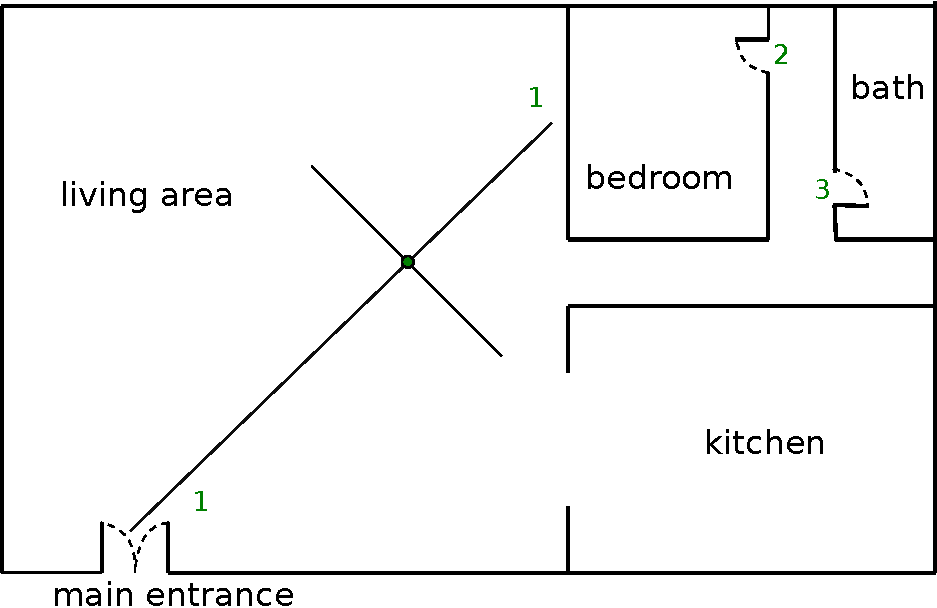
\includegraphics[width=65mm]{privacy-room-con}}
  \hspace{10 mm}
 \subfloat[Not Private]{\label{fig:private-room-incon}
\includegraphics[width=65mm]{privacy-room-incon}}
 \caption{Bedroom Privacy}
\label{room-privacy}
\end{figure}

Figure \ref{room-privacy} shows two example floor plans for a small single bedroom house; figure \ref{fig:private-room-con} shows a floor plan with a bedroom that is  private, while figure \ref{fig:private-room-incon} shows a similar floor plan with a bedroom that is not private. The numbers in the figures represent the following privacy requirements: (1) the bedroom is positioned on the opposing side of the building with regards to the main entrance, (2) the doorway is not visible from the main living space, and (3) the doorway is does not mutually face towards another doorway. Number that are in red indicate that the requirement has been broken, while numbers in green indicate that the requirement has been met.


\subsection{Continuity}
The concept of continuity in architecture describes a network of points that are mutually visible \cite{Key}. In DSpace, continuity is interpreted in the context of building navigation and wayfinding. Under this interpretation, a building, room or apartment is continuous if there is continuity between the doorways contained in the given space: room, building, or apartment. 

In DSpace, continuity is defined as a network of doorways that are mutually visible. The partitioning of doorways that should be mutually visible is based on a localized containment hierarchy of rooms and doorways, in which doorways that are contained in the same room should maintain continuity. It would not make sense for doorways that are located on opposite sides of a building to be visible to each other, but doorways that are in the same room should be. 

With respect to this definition, continuity is represented as a recursive predicate in Prolog, which takes a list of doorways and checks that each doorway is mutually visible to the others within the list. (need to mention doorways within a room). TBD: arguments: list of doors or room id that indicates containment level???

\begin{verbatim}
continuous([OBJ1,OBJ2|[]]) :- is_visible(OBJ1, OBJ2).

continuous([OBJ1,OBJ2|OBJS]) :- is_visible(OBJ1, OBJ2),
	                            is_visible(OBJ2, OBJ1),
                                continuity([OBJ1|OBJS]),
                                continuity([OBJ2|OBJS]).
\end{verbatim}

\begin{figure}[H]
 \centering
 \subfloat[Consistent]{\label{fig:continuity-con}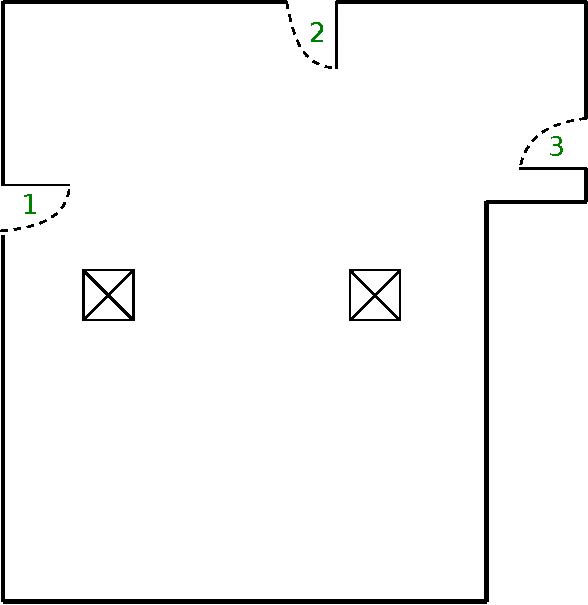
\includegraphics[width=45mm]{continuity-con}}
  \hspace{30 mm}
 \subfloat[Inconsistent]{\label{fig:continuity-incon}\includegraphics[width=45mm]{continuity-incon}}
 \caption{Continuity}
\label{continuity}
\end{figure}

Figure \ref{continuity} shows a floor plan for a single room with 3 doors. Figure \ref{fig:continuity-con} shows a configuration in which each door is mutually visible to the other doors. This design is consistent per the continuity requirement. Conversely, figure \ref{fig:continuity-incon} shows a configuration in which door 1 is not mutually visible to door 2 and door 1 is not mutually visible door 3. The visibility between door 1 and door 2 is obstructed by a column and the visibility between door 1 and door 3 is obstructed by a wall. Structural elements that are red indicated a visibility obstruction in-between doorways. This design does not met the continuity requirement. 


\subsection{Enclosure} 
The concept of enclosure in architecture defines a space, as experienced from a given vantage point, as being either confined or open. A confined space is defined as being confined by walls or columns, while an open space is defined as being spacious. In DSpace, enclosure is defined by localized spatial structures in terms of their proximity to a given point. Under this interpretation, a room, apartment, or building can be experienced as both confined and open based on the location of the vantage point within the space. Such a definition takes into account that enclosure is a locally experience. For example, an alcove in an otherwise open room, feels confined from the perspective of being inside the alcove.

In Dspace, a point is defined as open if less then three walls or columns are near-to the point. Conversely, a point is defined as confined if three or more walls or columns are near-to the point. While this interpretation of enclosure is naive, it maintains the notion that proximity defines the spatial structures of openness and confinement in a localized environment.   


\begin{verbatim}
confined(point) :-  

spacious(point) :-

\end{verbatim} 


Figure \ref{enclosure} shows a floor plan for a single room with various enclosure properties. The room has an alcove and a sequence of columns that will provide an environment of confinement. Points in-between the columns and inside the alcove are confined because of the proximity of multiple walls or columns. The points outside of these areas are open because there are no or few structures near by.


\begin{figure}[H]
\centering
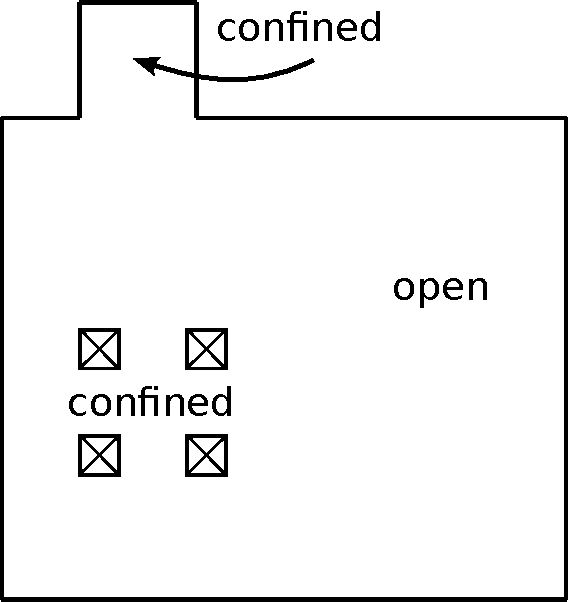
\includegraphics[width=50mm]{spacious-confined}
\caption{Enclosure, Confined and Open}
\label{enclosure}
\end{figure}


\subsection{Building Codes}
Building codes are a special case because they are precisely defined by an official body. 
 
In DSpace, security is defined by the doorways being observed by the a security camera \cite{Bhatt}. 

examples: camera range space door
          start landing
          sink bathroom
          


\section{Hierarchy}
Architectural concepts and qualitative spatial attributes are build on top of the physical / structural and artefactual geometries of the design in a hierarchical structure. Architectural concepts are defined by combining qualitative spatial attributes via the logical operators of conjunction and disjunction. The definition of an architectural concept is not limited to combining qualitative spatial attributes, spatial relationships of orientation, topology, and distance can be used as well as other geometric primitives such as area, angle, and length measurements. Similarly, qualitative spatial attributes in architecture are built by combining qualitative spatial relationships of orientation, topology, and distance. 

This design hierarchy is built on the discretion of a design space, quality space, and quantity space. The design space at the highest level, involves the architectural design semantics and qualities of architecture. The quantitative level is the lowest level that involves the precise geometries and structures of the design. The middle layer, the qualitative space, mediates the two via qualitative spatial representations of orientation, topology, and distance.

design space 
   architectural concepts
   spatial qualities of architecture
quality space
   qualitative spatial relations
   spatial abstractions
quantitative space
   structural geometry
   artefactual geometry
   
   
\begin{figure}[H]
\centering

\includegraphics[width=140mm]{hierarchy2}
\caption{Design Space Hierarchy}
\label{hierarchy}
\end{figure}

Figure \ref{hierarchy} shows the design hierarchy of the DSpace reasoner.



\chapter{Museum Case Study}
This chapter is a case study that demonstrates the application of the DSpace reasoner to the design of an art museum. The purpose is twofold: first, to examine several design requirements of an art museum with regards to the spatial interpretation of the requirements; and second, to show how the museum design requirements can be represented and reasoned about in a computational framework, in order to detect design inconsistencies as per the design requirements.

The remainder of the chapter is divided into three sections. The first section examines design requirements in art museums in three parts: the first part looks at requirements that influence museum visitors' behaviour. The second part looks at requirements for promoting exploration in the museum. The third part looks at the requirements of accessibility and security within the museum. The second section, looks at how these requirements can be interpreted spatially and represented in the DSpace reasoner. The third section tests the DSpace reasoner using sample museum floor plans that are both consistent and inconsistent per the design requirements for several art museums. The objective of this demonstration is to show that the DSpace reasoner can validate a design against its design requirements.



\section{Case Study Scenario: an art museum}
Museums are a place of public education, in which art, historical artefacts, and scientific exhibits are put on display for the public to view \cite{Falk}. While museums in general have many common threads in terms of their design requirements, this case study takes the approach of narrowing the study to that of an art museum. This focuses the discussion to specific real world examples and maintains the perspective that this is not an exhaustive study of museum design requirements, rather it's an investigation into the nature and interpretation, with respect to spatial properties / characteristics, of a set of design requirements. Additionally, the point is not to prove the validity of these requirements in an empirical sense; rather it is to show the process of representing and reasoning about design requirements in a formal computational framework.

The art museum is a unique and fruitful choice for this case study because it provides a rich set of design properties that have been formally studied and reported \cite{Melton} \cite{Bitgood02} \cite{Falk}. Within museum studies, visitor behaviour has been one of the primary focuses, starting with experiments dating back to the 1930's. 



\subsection{Museum Design Requirements}
Pretend for a moment that you are an architect working on the initial design for a new modern art museum. During your first visit with the museum's curator you discuss several design requirements that are important for the new museum. Your discussion reveals that the curator wants the new art museum to adhere to the following requirements:

\begin{enumerate}
\item Maximize visitor utilization of exhibitions
\item Encourage free-flowing exploration throughout the museum
\item Adhere to museum requirements of accessibility and security
\end{enumerate}

TBD: explain how these high level requirements can be interpreted into concrete properties of the museums design. from here the requirements can be spatially interpreted and represented in the DSpace reasoner.

\subsection{Maximizing Visitor Utilization of Exhibitions}
This portion of the case study will look into four factors that influence visitors' movement patters: positioning of doorways, spatial arrangement of display cases, positioning of furniture and statues, and congestion. These properties inform museum architects, during the design process, about the spatial characteristics that can maximize the utilization of the museum by increasing the frequency and duration with which visitors view exhibition objects. 

\subsubsection{Positioning of doorways}
In an important study, Melton \cite{Melton} discovered that the most influential factor to determine  the amount of attention an object receives is the object's position relative to doorways in a gallery room. Prior to this, museum researchers believed that the object's intrinsic properties of 'interestingness', color, and size were the real factors that determined the amount of attention an object received. Melton explained why this happens; he demonstrated that the amount of attention an object receives is directly related to the visitor circulation patterns within the museum and these circulation patterns emerge from the spatial characteristics of the museum's architecture.

\begin{figure}[H]
 \centering
 \subfloat[circulation pattern]{\label{fig:door-opposite}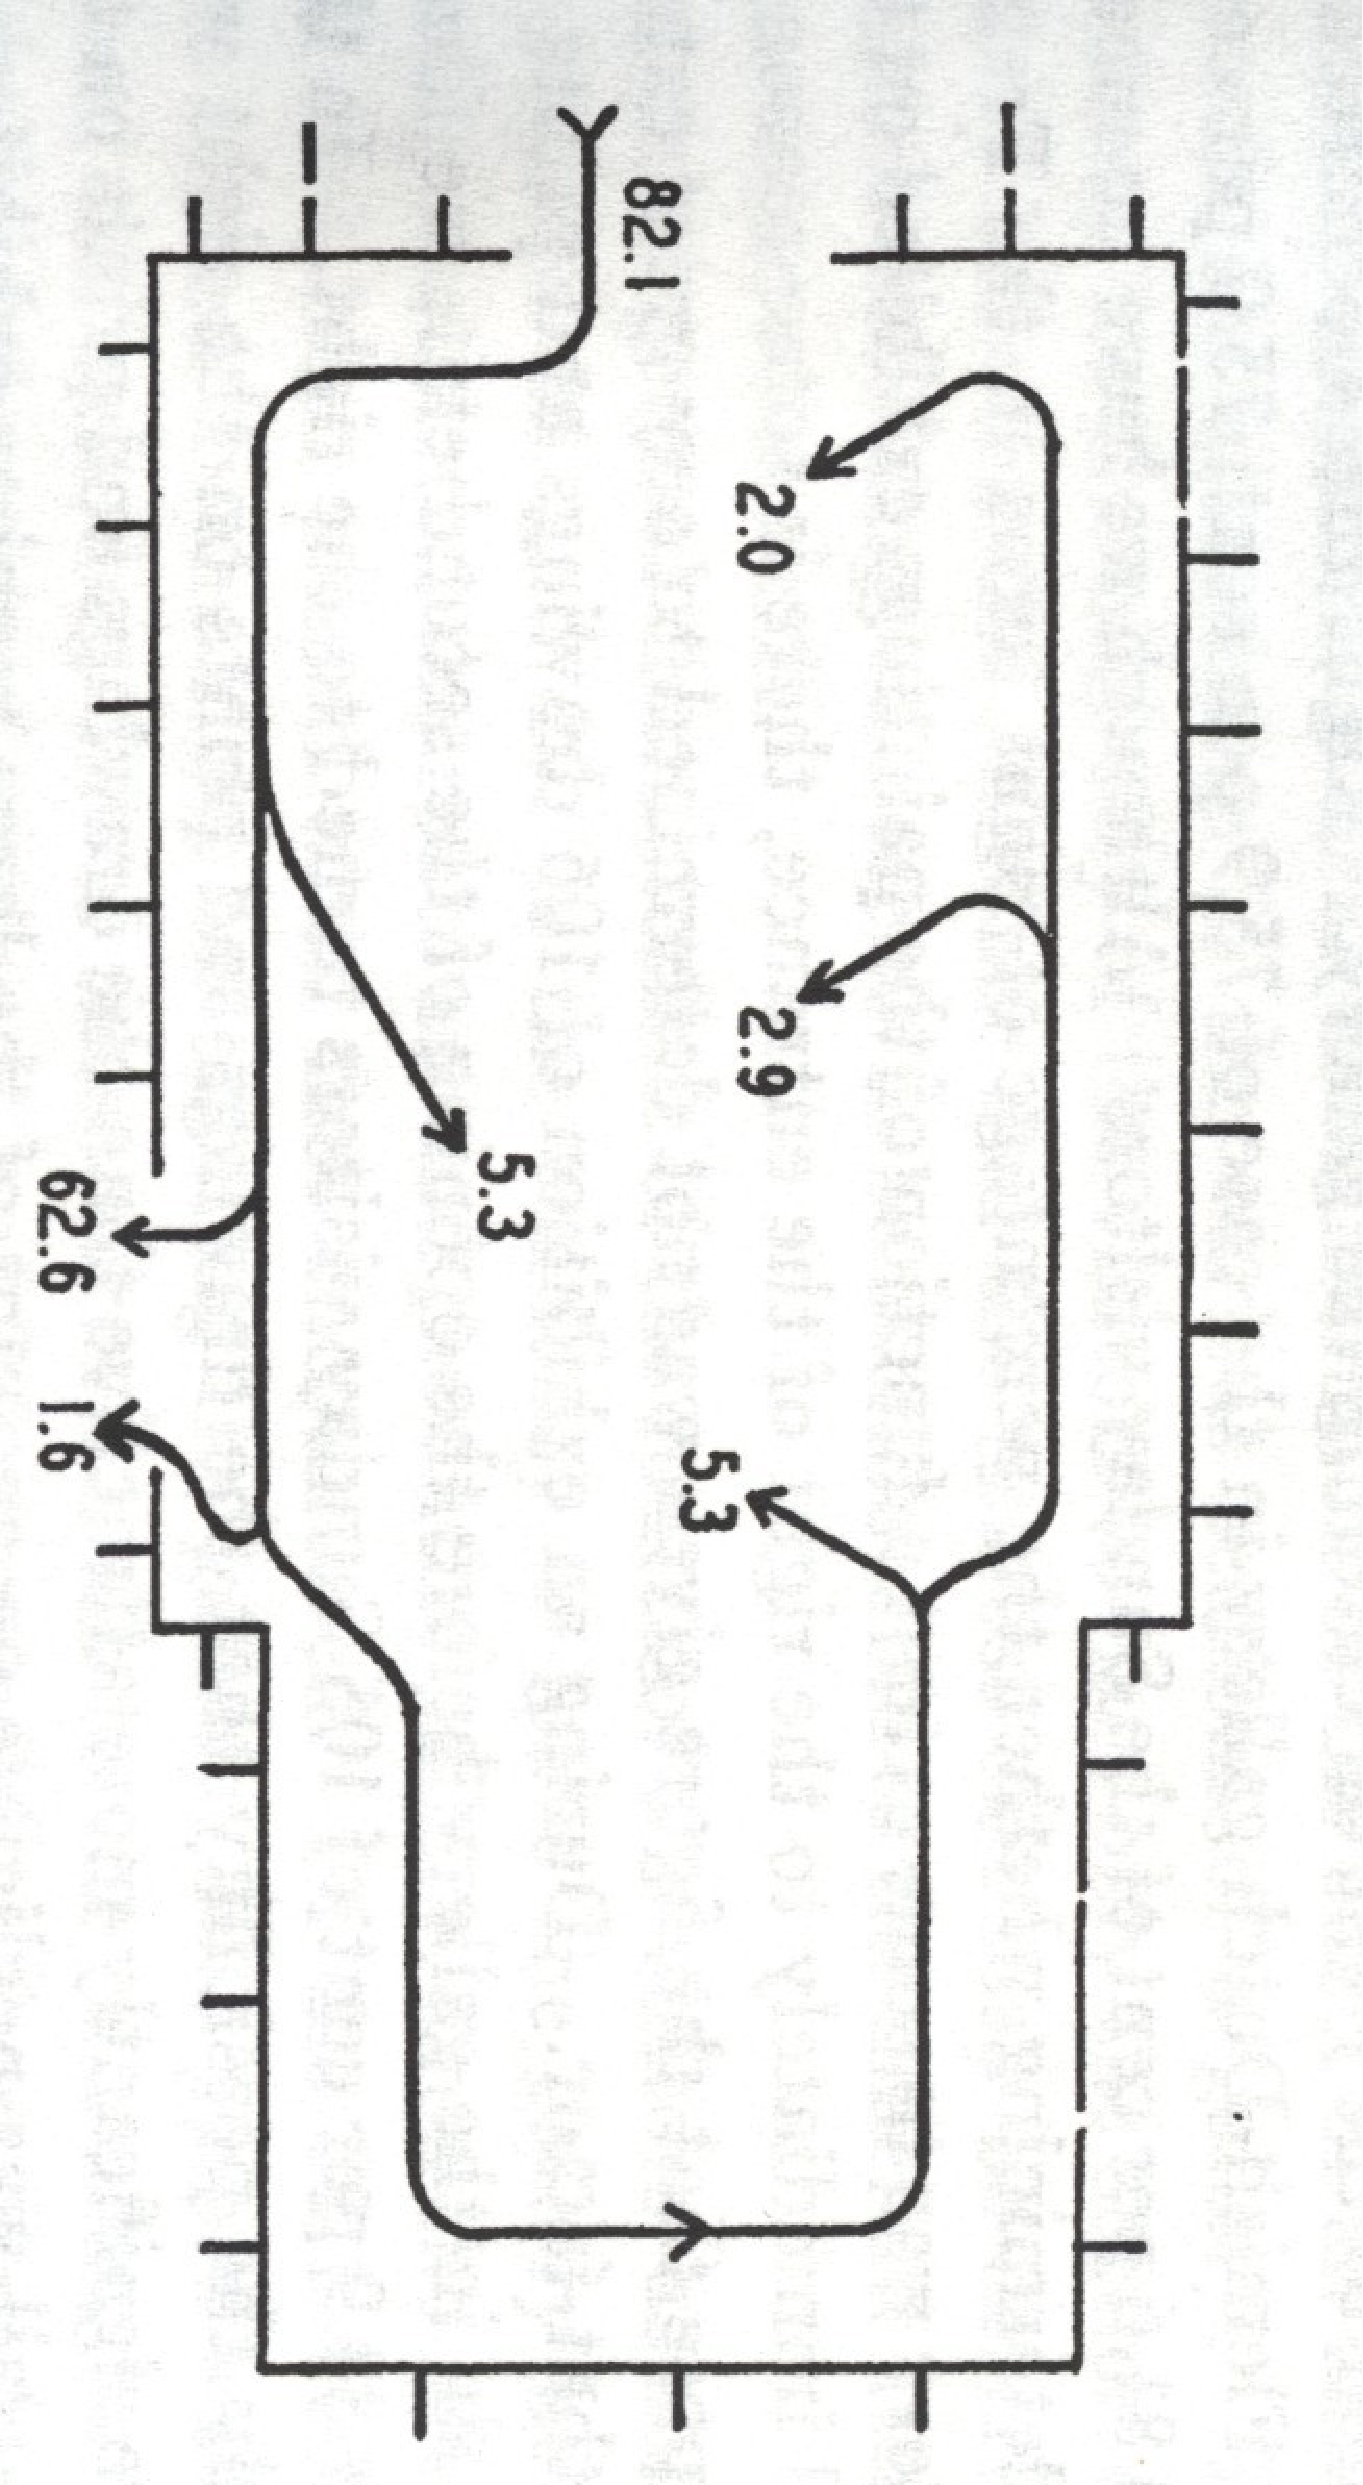
\includegraphics[width=35mm, angle=90]{melton-circulation}}
 \hspace{10 mm}
 \subfloat[frequency of visits]{\label{fig:door-opposite}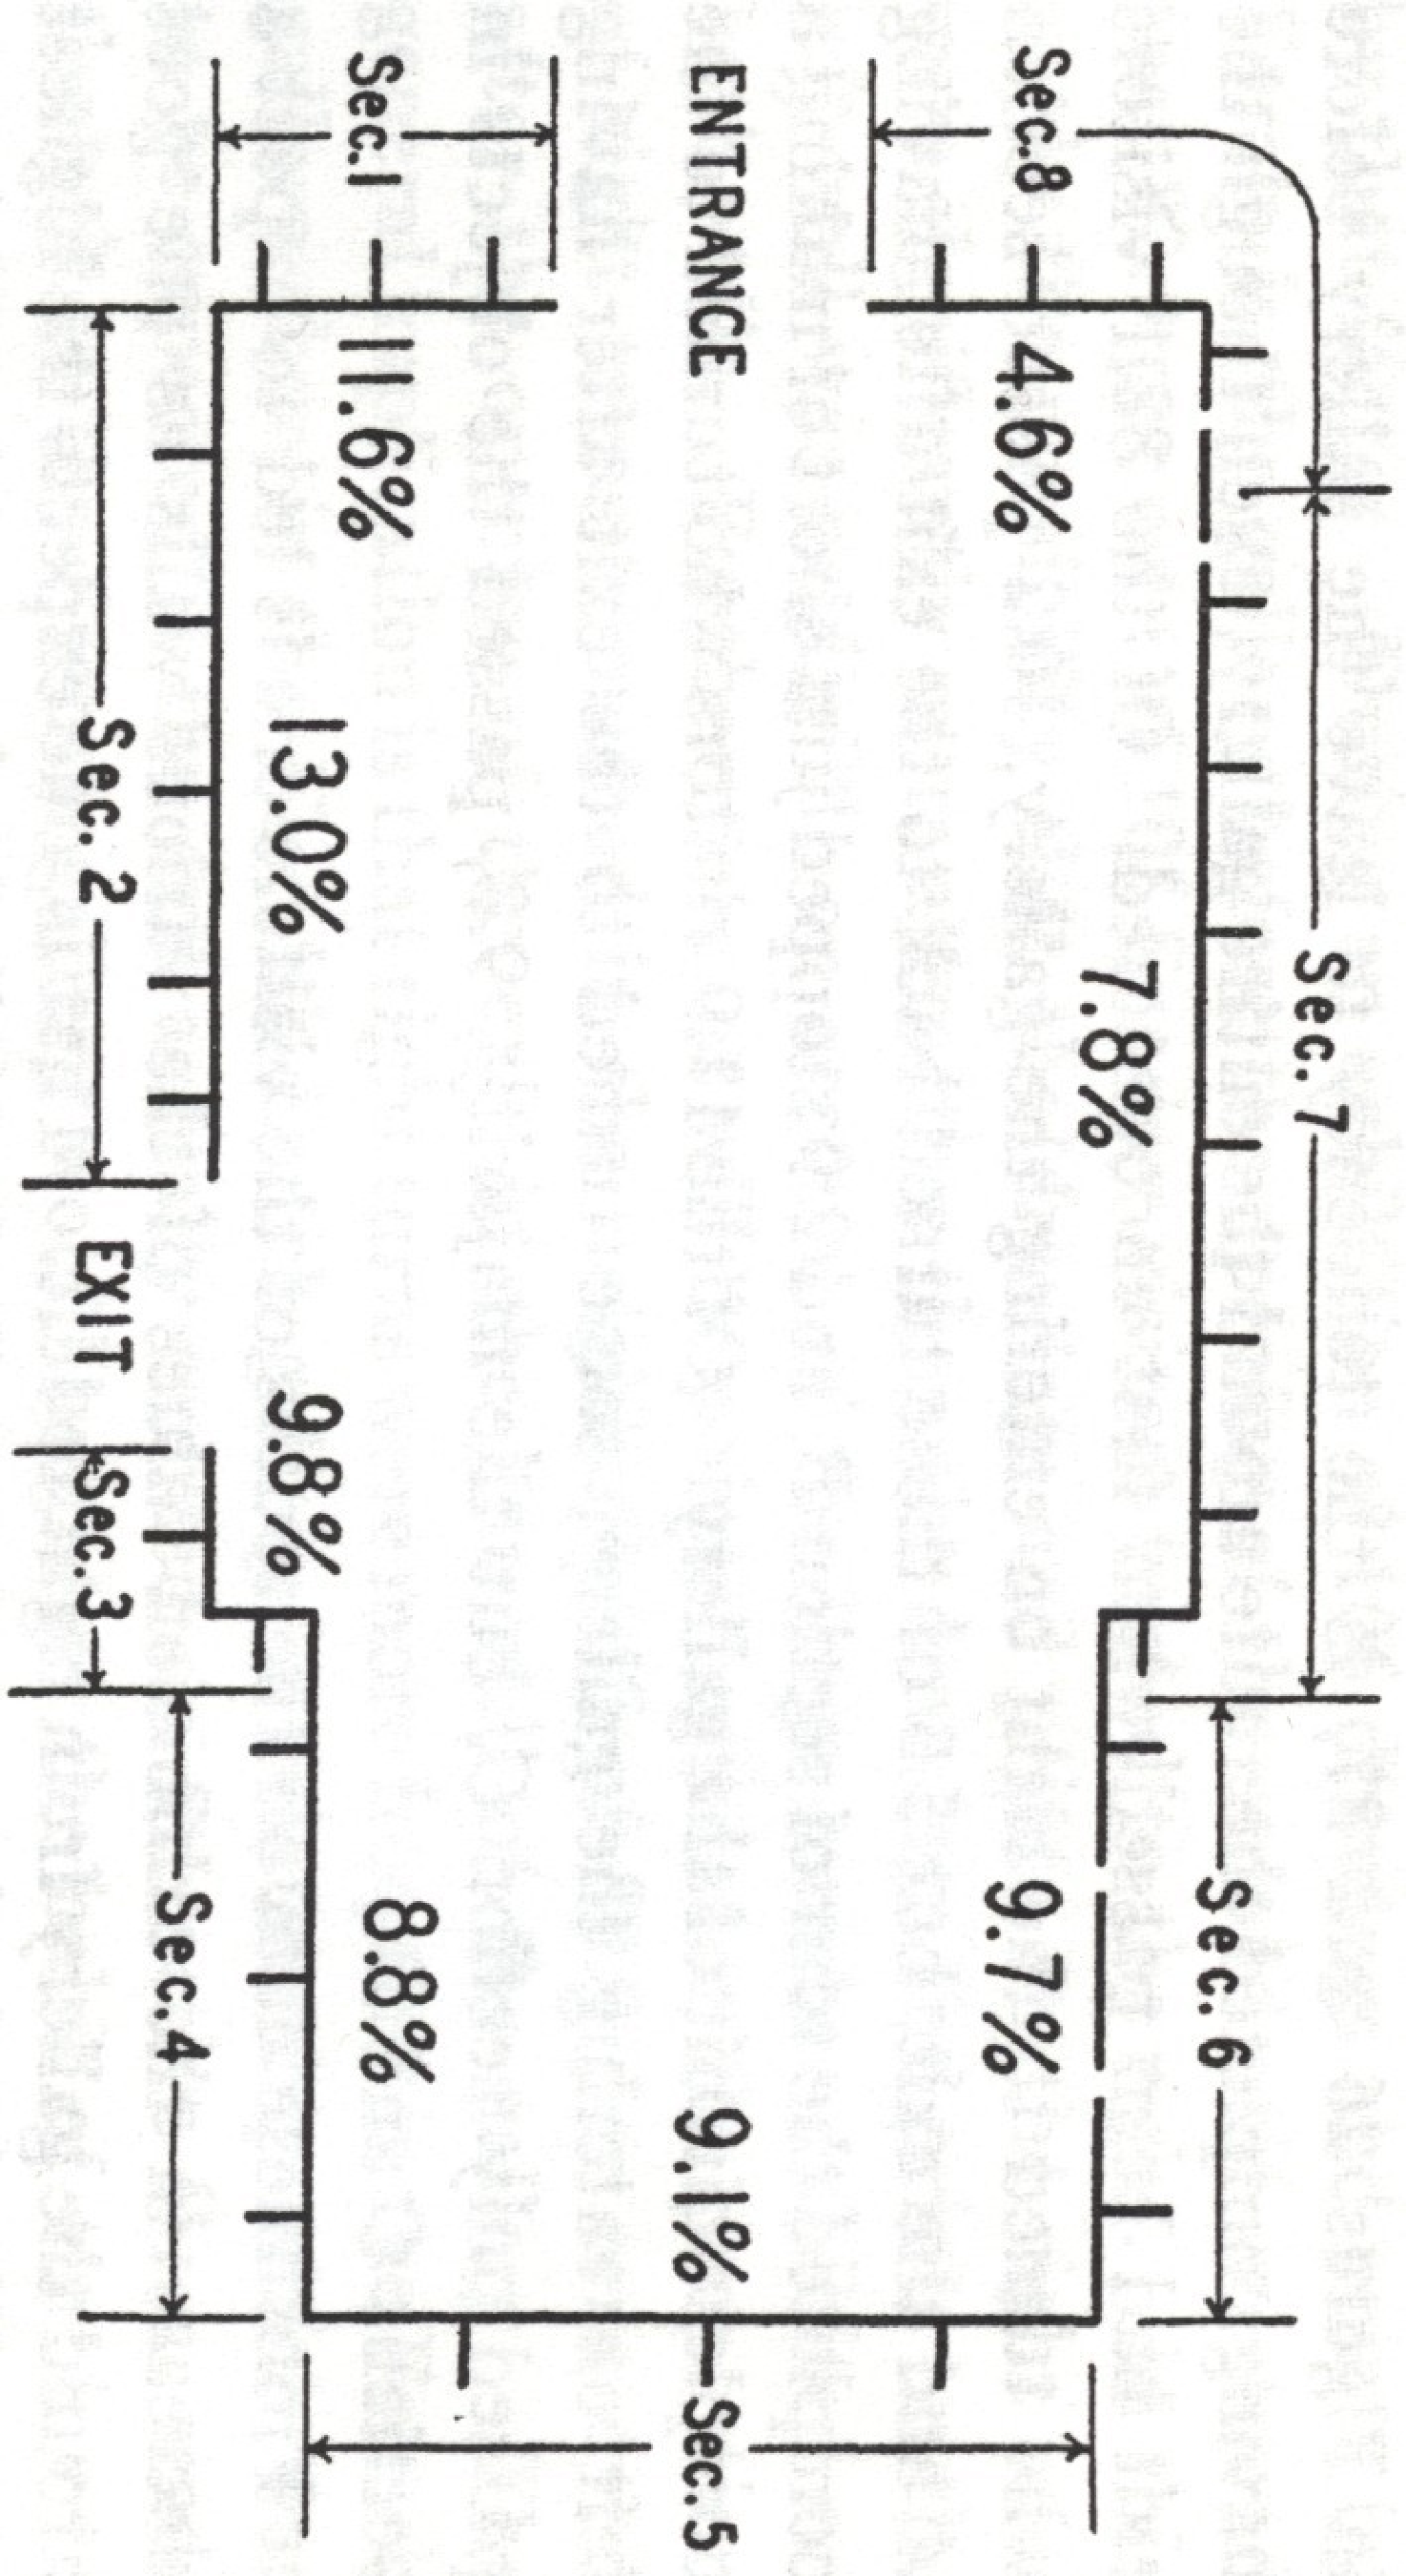
\includegraphics[width=35mm, angle=90]{melton-frequency}}
 \label{melton}
 \caption{Results from Melton's experiments on the effects of door positioning in an Art Museum}
\label{Melton-studies}
\end{figure}

The crux of Melton's experiments suggested that visitors exit through the first door they encounter, which he referred to as the exit gradient. Figure \ref{Melton-studies} shows the results of an extensive study of visitors circulation patterns and stopping frequencies in an art museum. The studies reported that almost 80 percent of visitors exited through the first exit they encountered before viewing the entire exhibition. Additionally, the studied showed that the most frequently visited objects where those located along the shortest path from the entrance to the exit. 

The results of Melton's studies inform architects of spatial characteristics that influence movement patterns in exhibitions. Specifically, doorways that are positioned on the same side of the room cause visitors to pay attention to fewer exhibits than doorways that are positioned on opposing sides of the room.

\begin{description}
\item[Requirement 1:] Exhibition doorways should be positioned on opposing sides of gallery rooms. 
\end{description}

Figure \ref{door-position} shows a possible exhibition design where the red door is positioned on the same side of the room as the entrance, while the black door is positioned on the opposing side.
\begin{figure}[H]
\centering
\subfloat[consistent design]{\label{fig:door-opposite}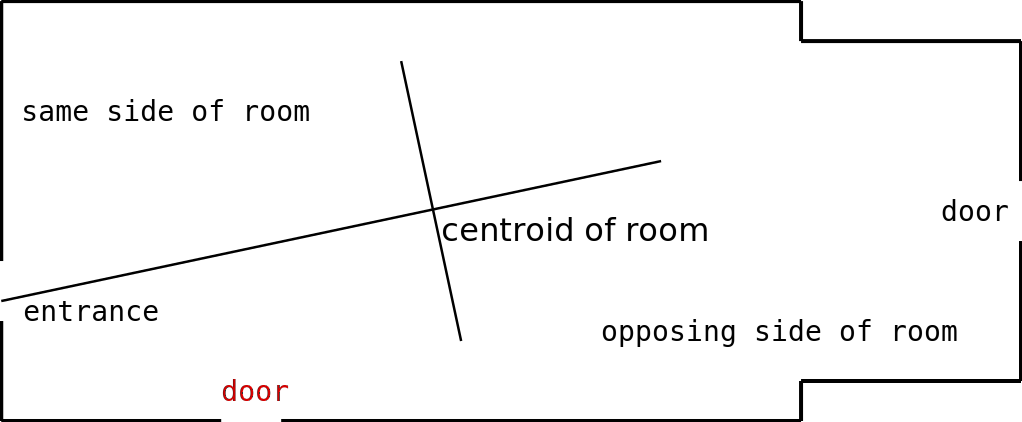
\includegraphics[width=85mm]{door-possitioning}}
\caption{Schematization of the opposing door requirement.}
\label{door-position}
\end{figure}

Bitgood suggests that visitors tend to follow along the wall that is closest to the door they entered \cite{Bitgood95}. Given that visitors also tend to exit through the first doorway they encounter, doorways should not be positioned in a wall that is adjacent to another doorway.  
 
\begin{description}
\item[Requirement 2:] Exhibition doorways should not be positioned on a wall that is adjacent to another doorway.
\end{description}


\subsubsection{Spatial arrangement of display cases}
The spatial arrangement of display cases in galleries has been shown to influence visitors' movement patterns. \cite{Bitgood92} showed that display case arrangements that form a perimeter or a peninsula generate the most amount of attention, while display case arrangements that form an island in the middle of the room received the lowest amount of attention.

   \begin{figure}[H]
 \centering
 \subfloat[island]{\label{fig:door-opposite}
\includegraphics[width=35mm]{island}}
 \hspace{10 mm}
 \subfloat[perimeter]{\label{fig:door-opposite}
\includegraphics[width=35mm]{perimeter}}
  \hspace{10 mm}
 \subfloat[peninsula]{\label{fig:door-opposite}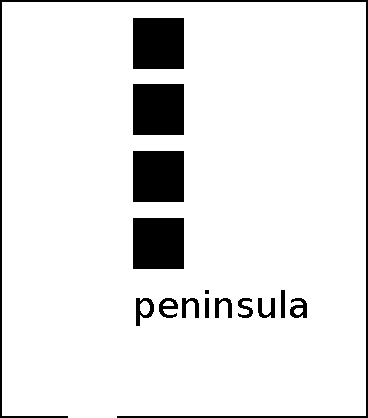
\includegraphics[width=35mm]{peninsula}}
 \caption{Display case arrangements}
\label{display-arrangement}
\end{figure}
 
\begin{description}
\item[Requirement 3:] Display case arrangements should not form an island near the center of the room.
\end{description} 

Circulation patterns can be disrupted when a peninsula arrangement cuts horizontally across the view of a visitor as they are entering the room. This type of display pattern will cut off part of the room from the visitor and will make it less likely to be visited.

\begin{description}
\item[Requirement 4:] Display cases arrangements that form a peninsula should not cut horizontally across the view of a visitor located at an entrance.
\end{description} 

\begin{figure}[H]
\centering
\subfloat[consistent design]{\label{fig:door-opposite}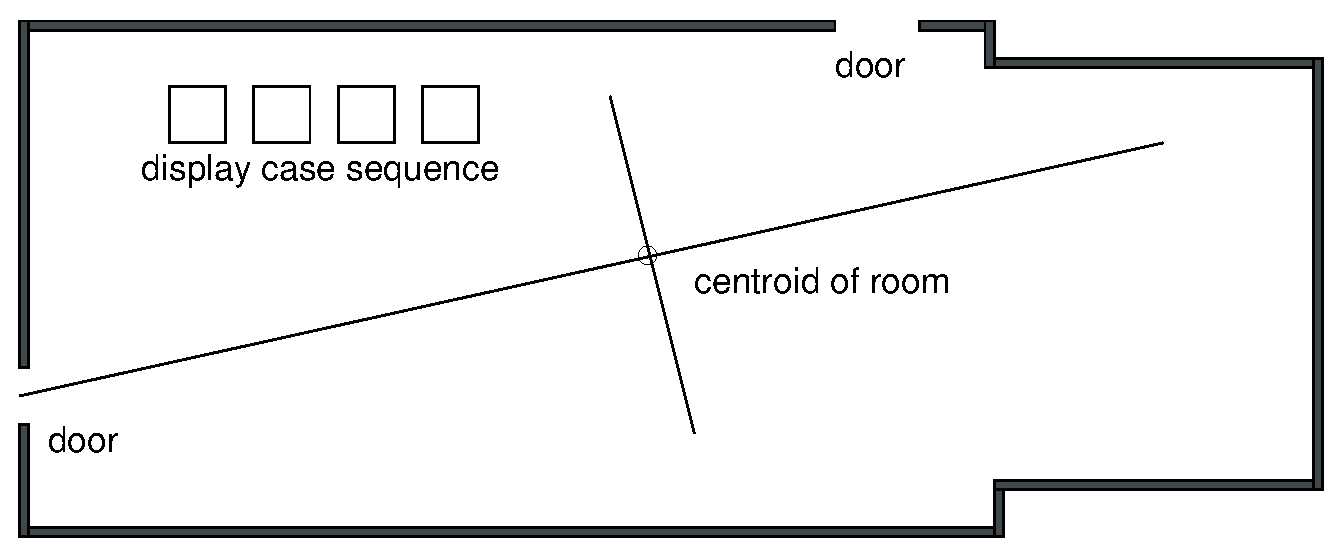
\includegraphics[width=65mm]{display-not-cut}}
\hspace{10 mm}
\subfloat[inconsistent design]{\label{fig:door-opposite}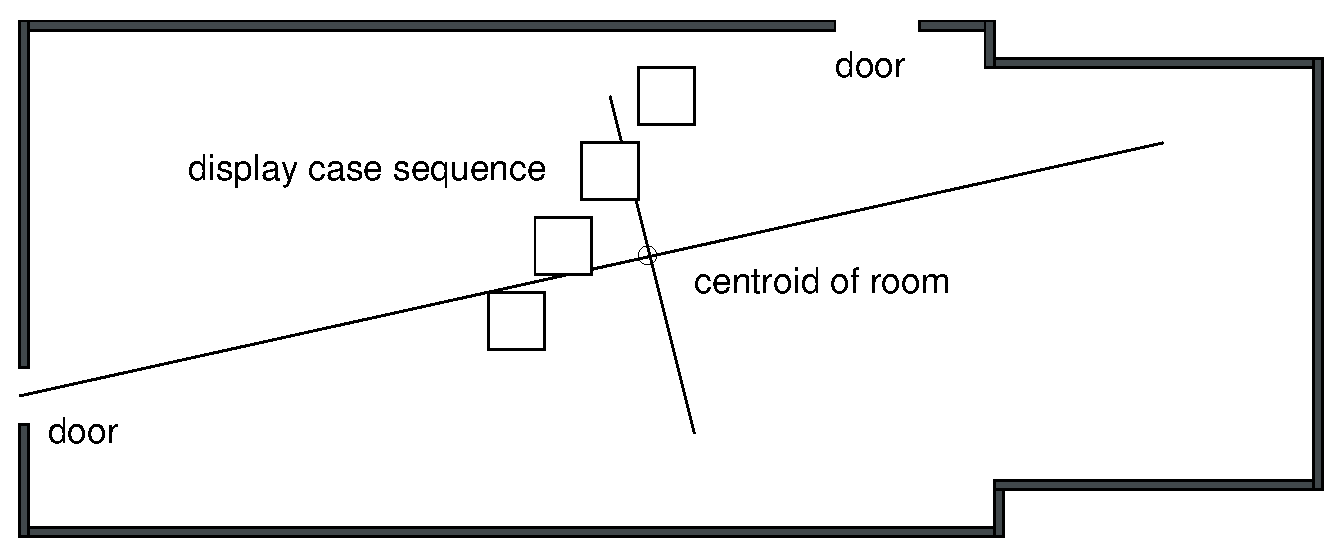
\includegraphics[width=65mm]{door-cut-room}}
\end{figure}


\subsubsection{Congestion}
Congestion in museums can be caused by interference of displayed objects and their viewing spaces with movement pathways of visitors. In order to reduce congestion in museums, designers should be aware of the placement of display cases, statues, furniture (seating benches), and information kiosks within the gallery. The following are requirements that should be followed to reduce congestion in museums:

\begin{description}
\item[Requirement 5:] The viewing area of display cases, functional space of doors, function space of seating areas, and operation space of information kiosks should not interfere with each other.
\end{description}

\subsubsection{Positioning of benches, statues, and information kiosks}
The positioning and orientation of benches and statues can increase the amount of attention an exhibition receives and change circulation patterns within a gallery \cite{Stavroulaki} \cite{Museum}. Studies have shown that seating directly facing an object will increase the attention the object receives, even if no one uses the seating. 

\begin{description}
\item[Requirement 6:] Seating should directly face a gallery wall or display case.
\end{description}

The orientation of a statue to doorways can increase the attention the statue receives as well as the object close to it. Statues that face away from doorways encourage visitors to move around the statues in order to get a better view.  
\begin{description}
\item[Requirement 7:] Statues should face away from doorways.
\end{description}

\subsubsection{Visitor Orientation in the lobby}
The lobby is the first place visitors encounter when they enter a museum. The design of the lobby is important because it not only provides a first glimpse of the museum's exhibits but it is the place where the museum provides services to its visitors, including: a ticketing desk, bathrooms, an information desk, and entrances to exhibitions \cite{Bitgood02}. The aim of the requirements for the lobby focus on making it easy for visitors to locate services and orient themselves to the new environment. 

Upon entering the lobby most visitors need to find the ticket area and/or an information desk. It is important, therefore, that the ticketing area and information desk are visible from the entrance. If there is more then one entrance, then it is important that the ticket area and information desk are visible from all entrances. 

\begin{description}
\item[Requirement 8:] The ticketing and information desks should be visible from the main entrance(s).
\end{description}

Additionally, studies have shown that people first look to their right hand side when entering a building. By placing the ticket and information desks on the right hand side of the lobby, visitors are more likely to notice them immediately when they enter the lobby. 

\begin{description}
\item[Requirement 9:] The ticketing area should be on the right side of the lobby from the main entrance(s).
\end{description}

The ticketing area should be close to visitors when they enter because it is likely one of the first places they will need to visit.
\begin{description}
\item[Requirement 10:] The ticketing are should be on the same side of the lobby as the entrance(s).
\end{description}

Bathrooms are an important services for museum visitors. Surprisingly, the place of the bathroom can have an impact on how long visitors stay in the museum. Studies \cite{tbd} have found that bathrooms that are located on the same side of the lobby as the entrance / exit encourage visitors to leave earlier compared to museums with bathrooms on the opposing side of the lobby from the entrance / exit. 

\begin{description}
\item[Requirement 11:] The bathroom should be on the opposing side of the lobby from the entrance / exit.
\end{description}

The doors should be private to maintain as much privacy in the bathrooms as possible.

\begin{description}
\item[Requirement 12:] Bathroom doors should be private.  
\end{description}

The main exhibition entrance should be clearly visible from several parts of the lobby to make it easy for visitors to find where they need to go. 
\begin{description}
\item[Requirement 13:] Exhibit entrance should be visible from the ticketing area and central lobby location
\end{description}


\subsection{Exploration}
The way visitors explore an exhibition is influenced by the spatial characteristics of the layout, as well as the characteristics of each gallery room. Layouts that are sequential, i.e. one way in / one way out, promote a controlled and orderly flow of movement. Museums of history and science are well served by this type of design because they have a narrative to tell that is chronological. On the other hand, layouts that present the visitor with path choices, i.e. multiple doorways, promote free-flowing exploration. In this type of layout it is important that visitors are aware of the path choices that are available. This means that doorways are visible between each other throughout the layout. This concept of visibility between a network of points is referred to as continuity and is an important characteristic of layouts that present visitors with multiple path choices.  

\begin{description}
\item[Requirement 14:] The layout of the museum should maintain continuity between doorways within each exhibition and gallery room.
\end{description}

Within a Gallery, rooms that are open promote more free-flowing exploration than rooms that are narrow. Narrow rooms inhibit exploration because of space limitations and confinement. Rooms that are open provide more space for visitors to explore the room in a free-flowing manner.
\begin{description}
\item[Requirement 15:] Gallery rooms should be open, rather than narrow, in order to promote free-flowing exploration.
\end{description}


\subsection{Accessibility and Security}
Museums should be accessible and easy to navigate. TBD - I have some ideas here but nothing concrete. Maybe you have some ideas that you can share with me. 
\begin{description}
\item[Requirement 16:] Museums should be accessible.
\end{description}
Museums should be secure.
\begin{description}
\item[Requirement 17:] The functional space of every gallery doorway should overlap with the range space of at least one security camera.
\end{description}


\section{Representation and Reasoning for Museums of Art in DSpace} 


\subsection{Representation}

\subsubsection{Spatial Interpretation of a Design Requirement}

\subsubsection{Using the Building Blocks from DSpace}

\subsection{Case Study Tests}

\subsubsection{ArchiCAD / IFC}

\subsubsection{Detecting Inconsistent and Consistent Designs}

\chapter{Evaluation}


\chapter{Future Work / Conclusion}



% ------------- End main chapters ----------------------

\clearpage
\bibliographystyle{abbrv}
\bibliography{museum}
\bibliography{design}
%\addcontentsline{toc}{chapter}{Bibliography}

\end{document}